\begin{tikzpicture}[]

  \tikzstyle{netstyle} = [matrix of nodes,nodes={draw,rectangle,inner sep=0, minimum size=1.5cm, anchor=center},column sep=0.2pt,row sep=0.2pt]
  \tikzstyle{zentral} = [fill=red!70!pagecolor]

  \matrix[netstyle] (mat)
  {
    $(\mat{F})_{1,1}$ & $(\mat{F})_{1,2}$ & $(\mat{F})_{1,3}$\\
    $(\mat{F})_{2,1}$ & |[zentral]|$(\mat{F})_{C}$ & $(\mat{F})_{2,3}$\\
    $(\mat{F})_{3,1}$ & $(\mat{F})_{3,2}$ & $(\mat{F})_{3,3}$\\
  };

  \draw[<->, thick,transform canvas={xshift=-3mm}] (mat-3-1.south west) -- (mat-1-1.north west) node [midway,sloped,above] {$f$};
  \draw[<->, thick,transform canvas={yshift=-3mm}] (mat-3-1.south west) -- (mat-3-3.south east) node [midway,sloped,below] {$f$};
\end{tikzpicture}

\begin{tikzpicture}[every node/.style={minimum size=1cm},on grid]

  % left front
  \begin{scope}[every node/.append style={yslant=-0.5},yslant=-0.5]
    \shade[right color=gray!10, left color=black!50] (0,0) rectangle +(3,3);
    \node at (0.5,2.5) {$(\mat{F})_{1,1,1}$};
    \node at (1.5,2.5) {7};
    \node at (2.5,2.5) {1};
    \node at (0.5,1.5) {2};
    \node at (1.5,1.5) {4};
    \node at (2.5,1.5) {8};
    \node at (0.5,0.5) {5};
    \node at (1.5,0.5) {3};
    \node at (2.5,0.5) {6};
    \draw (0,0) grid (3,3);
  \end{scope}

  % right front
  \begin{scope}[every node/.append style={yslant=0.5},yslant=0.5]
    \shade[right color=gray!70,left color=gray!10] (3,-3) rectangle +(3,3);
    \node at (3.5,-0.5) {3};
    \node at (4.5,-0.5) {we};
    \node at (5.5,-0.5) {7};
    \node at (3.5,-1.5) {6};
    \node at (4.5,-1.5) {1};
    \node at (5.5,-1.5) {5};
    \node at (3.5,-2.5) {8};
    \node at (4.5,-2.5) {2};
    \node at (5.5,-2.5) {4};
    \draw (3,-3) grid (6,0);
  \end{scope}

  % top
  \begin{scope}[every node/.append style={
      yslant=0.5,xslant=-1},yslant=0.5,xslant=-1
    ]
    \shade[bottom color=gray!10, top color=black!80] (6,3) rectangle +(-3,-3);
    \node at (3.5,2.5) {1};
    \node at (3.5,1.5) {4};


    \node at (3.5,0.5) {7};
    \node at (4.5,2.5) {5};
    \node at (4.5,1.5) {6};
    \node at (4.5,0.5) {8};
    \node at (5.5,2.5) {2};
    \node at (5.5,1.5) {3};
    \node at (5.5,0.5) {he};
    \draw (3,0) grid (6,3);
  \end{scope}
\end{tikzpicture}



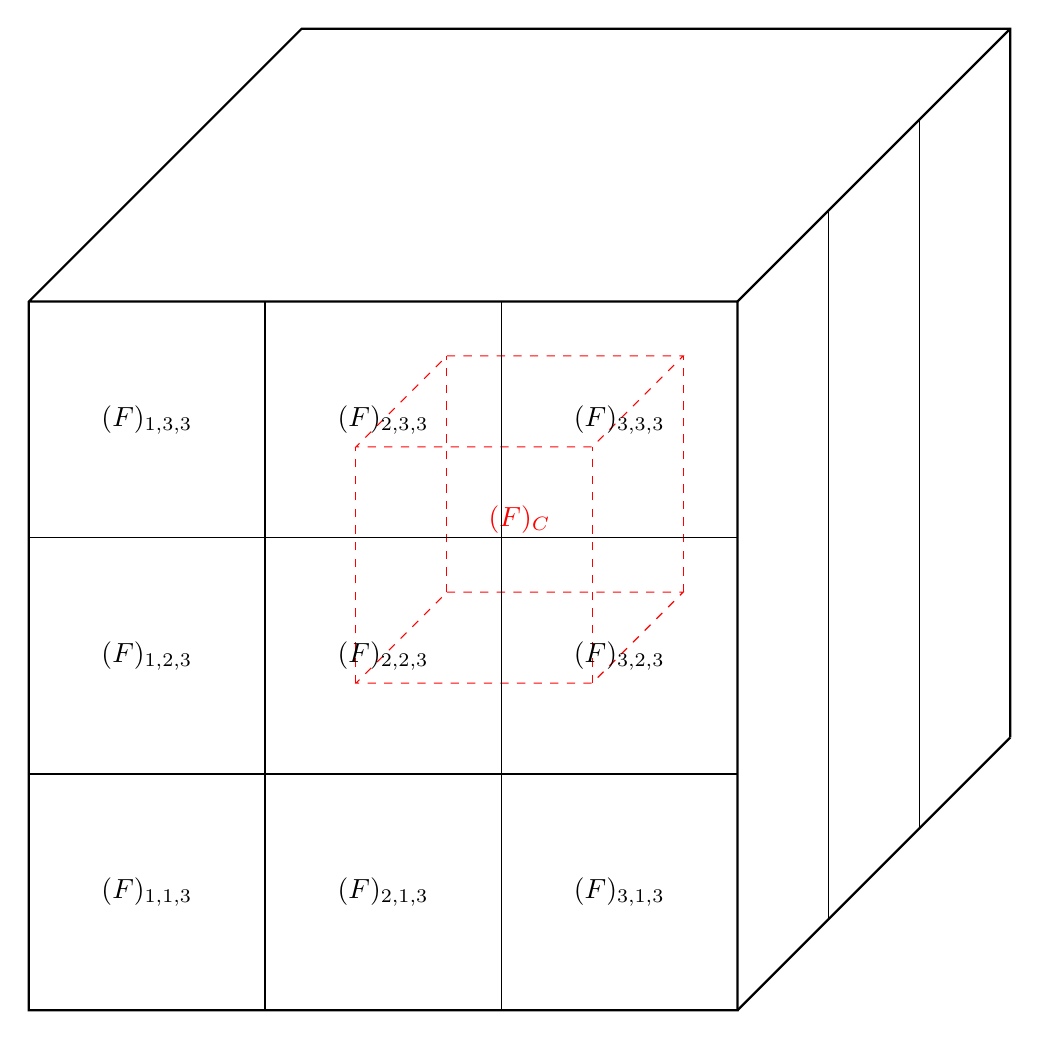
\begin{tikzpicture}%[x={(0.866cm,0.5cm)}, y={(-0.866cm,0.5cm)}, z={(0cm,1cm)}, scale=0.7]
  \draw[thick] (9,0,0) coordinate (x) |- (0,9,0) coordinate [midway] (h) coordinate (y) -- (0,9,9) coordinate (a) -- (0,0,9) coordinate (z) -- (9,0,9) edge (x) -- (9,9,9) coordinate (v) edge (h)
  -- (a);
  % \draw [dashed] (0,0,0) coordinate (o) edge (x) edge (y) -- (z);


  % zentralelement
  \draw [dashed, red] (3,6,3) -- ++(3,0,0) -- ++(0,0,3) -- ++(-3,0,0) -- ++(0,0,-3); % top
  \draw [dashed,red] (3,3,3) -- ++(3,0,0) -- ++(0,0,3) -- ++(-3,0,0) -- ++(0,0,-3); % bottom
  \draw [dashed, red] (3,3,3) -- (3,6,3) (3,3,6) -- (3,6,6) (6,3,3) -- (6,6,3) (6,3,6) -- (6,6,6); % connecting

  \foreach \x/\xt in {1.5/1,4.5/2,7.5/3} {
    \foreach \y/\yt in {1.5/1,4.5/2,7.5/3} {
      \coordinate (pos) at (\x,\y,9);
      \node [] at (pos) {$(\ten{F})_{\xt,\yt,3}$};
    }
  }
  \node [red,fill=white] at (4.5, 4.5, 4.5) {$(\ten{F})_C$};

  \foreach \c in {3,6} {
    % front
    \draw [] (\c,0,9) -- (\c,9,9);
    \draw [] (0,\c,9) -- (9,\c,9);

    % right
    \draw [] (9,0,\c) -- (9,9,\c);
  }
    \foreach \y/\yt in {3,6} {
      \foreach \z/\zt in {3,6} {
      }
    }


\end{tikzpicture}


\begin{tikzpicture}[x={(0.866cm,0.5cm)}, y={(-0.866cm,0.5cm)}, z={(0cm,1cm)}, scale=0.7]

  \begin{scope}[canvas is xz plane at y=0,transform shape]
    \foreach \ii [count = \xi] in {-3,-2,...,3}{
      \foreach \jj  [count = \yi] in {-3,-2,...,3}{
        \pgfmathsetmacro{\num}{int(abs(\ii)+abs(\jj))}
        \node[draw=blue!20!pagecolor,fill=blue!2!pagecolor,text=textcolor,minimum size=1cm] (n-1-\xi-\yi) at (\xi,-\yi) {\LARGE \num};
      }
    }
    \foreach \ii [count = \xi] in {-3,-2,-1}{
      \foreach \jj [count = \yi] in {-3,-2,-1}{
        \pgfmathsetmacro{\num}{int(abs(min(\ii,\jj))}
        \node[draw=blue!20!pagecolor,fill=blue!10!pagecolor,minimum size=1cm] (n-1-\xi-\yi) at (\xi,-\yi) {\LARGE \num}; % rename nodes
      }
    }

    \path[draw=black,thick] (n-1-1-1.north west) -- (n-1-7-1.north east) -- (n-1-7-7.south east) -- (n-1-1-7.south west) -- cycle;
    \path[draw=blue] (n-1-1-1.north west) -- (n-1-3-1.north east) -- (n-1-3-3.south east) -- (n-1-1-3.south west) -- cycle;


  \end{scope}

  \begin{scope}[canvas is xz plane at y=-7.3,transform shape]
    \foreach \ii [count = \xi] in {-1,0,1}{
      \foreach \jj  [count = \yi]in {-1,0,1}{
        \pgfmathsetmacro{\num}{int(\ii)}
        \node[draw=blue!20!pagecolor,fill=blue!10!pagecolor,text=textcolor,minimum size=1cm] (n-2-\xi-\yi) at (\xi,-\yi) {\LARGE \num};
      }
    }

    \path[draw=blue] (n-2-1-1.north west) -- (n-2-3-1.north east) -- (n-2-3-3.south east) -- (n-2-1-3.south west) -- cycle;
  \end{scope}

  \begin{scope}[canvas is xz plane at y=-11.2,transform shape]
    \foreach \ii [count = \xi] in {1,2,3,...,7}{
      \foreach \jj  [count = \yi]in {1,2,3,...,7}{
        \node[draw=blue!20!pagecolor,fill=blue!2!pagecolor,text=textcolor,minimum size=1cm] (n-3-\xi-\yi) at (\xi,-\yi) {};
      }
    }

    \foreach \ii [count = \xi] in {-3,-2,-1}{
      \foreach \jj [count = \yi] in {-3,-2,-1}{
        \pgfmathsetmacro{\num}{int(abs(min(\ii,\jj))}
        \node[draw=blue!20!pagecolor,fill=blue!10!pagecolor,minimum size=1cm] (n-3-\xi-\yi) at (\xi,-\yi) {}; % rename nodes
      }
    }

    \path[draw=blue,dashed] (n-3-1-1.north west) -- (n-3-3-1.north east) -- (n-3-3-3.south east) -- (n-3-1-3.south west) -- cycle;
    \path[thick,draw=black] (n-3-2-2.north west) -- (n-3-6-2.north east) -- (n-3-6-6.south east) -- (n-3-2-6.south west) -- cycle;
  \end{scope}

  % red box
  \path[draw=red,fill=red!50,opacity=0.3] (n-1-2-2.north east) -- (n-2-2-2.north east) -- (n-3-2-2.north east) -- (n-3-2-2.north west) -- (n-2-2-2.north west) -- (n-1-2-2.north west); % top
  \path[draw=red,fill=red!50,opacity=0.3] (n-1-2-2.south east) -- (n-2-2-2.south east) -- (n-3-2-2.south east) -- (n-3-2-2.south west) -- (n-2-2-2.south west) -- (n-1-2-2.south west); % bottom
  \path[draw=red,fill=red!50,opacity=0.3] (n-1-2-2.north east) -- (n-2-2-2.north east) -- (n-3-2-2.north east) -- (n-3-2-2.south east) -- (n-2-2-2.south east) -- (n-1-2-2.south east); % right
  \path[draw=red,fill=red!50,opacity=0.3] (n-1-2-2.north west) -- (n-2-2-2.north west) -- (n-3-2-2.north west) -- (n-3-2-2.south west) -- (n-2-2-2.south west) -- (n-1-2-2.south west); % left


  % blue lines connecting
  \path[draw=blue!40!pagecolor] (n-1-1-3.south west) -- (n-2-1-3.south west) -- (n-3-1-3.south west);
  \path[draw=blue!40!pagecolor] (n-1-3-1.north east) -- (n-2-3-1.north east) -- (n-3-3-1.north east);

  \begin{scope}[canvas is xz plane at y=0,transform shape]
    \node[yshift=1.2cm,black] (rf-tag) at (n-1-4-1.north) {\LARGE ursprüngliches Bild $\mat{B}$};
    \node[draw=red,minimum size=1cm] (marked1) at (2,-2) {\LARGE 2};
    \node[yshift=0.5cm,blue] (rf-tag) at (n-1-2-1.north) {\large Rezeptives Feld $\hat{\mat{B}}^{(2,2)}$};
    \node[xshift=-0.5cm,red,rotate=90] (rf-tag) at (n-1-1-2.west) {\large Quellenpixel $(\mat{B})_S$};
  \end{scope}

  \begin{scope}[canvas is xz plane at y=-7.3,transform shape]
    \node[draw=red,text=textcolor,minimum size=1cm] (marked2) at (2,-2) {\LARGE 0};
    \node[yshift=0.5cm,blue] (rf-tag) at (n-2-2-1.north) {\large Filter $\mat{F}$};
    \node[xshift=-0.5cm,red,rotate=90] (rf-tag) at (n-2-1-2.west) {Zentralelement $(\mat{F})_C$};
  \end{scope}

  \begin{scope}[canvas is xz plane at y=-11.2,transform shape]
    \node[yshift=0.5cm,black] (rf-tag) at (n-3-4-2.north) {\LARGE neues Bild $\tilde{\mat{B}}$};
    \node[draw=red,fill=blue!10!white,text=textcolor,minimum size=1cm] (marked3) at (2,-2) {\LARGE -3};
  \end{scope}

\end{tikzpicture}

%%% Local Variables:
%%% mode: latex
%%% TeX-master: "../figs"
%%% End:
